\section{Setup}
\label{sec:setup}

\begin{table}[H]
\centering\small
\caption{Assignment and tools.}
\begin{tabular}{lp{11.2cm}}
\toprule
Item & Value \\
\midrule
Model file & \texttt{models/32nm\_MGK.pm} (BSIM4, level 54), used unchanged; SHA256 {\small\path{56710120d5a2ae9e32a1908e1ee29a98f692a1dec0501eed8976ea6e6bea021e}} \\
Simulator & ngspice 42; model level=54, version=4.0, handled by the ngspice BSIM4v5 implementation \\
Solver options & gmin=1e-18, abstol=1e-18\,A, reltol=1e-6, vntol=1e-9\,V (in every deck) \\
Supply and temperature & $V_{DD}$ nominal \SI{0.9}{\volt}, sampled \SIrange{0.81}{0.99}{\volt}; temperature $-40$ to \SI{125}{\celsius}, model nominal \SI{27}{\celsius} \\
Channel length $L$ & \SI{32}{\nano\meter} \\
Nominal supply & $V_{DD}=\SI{0.9}{\volt}$ \\
Test circuit & 8-bit parity checker: 7 XOR gates $\times$ 4 NAND2 $=$ 28 NAND2, 112 MOSFETs \\
Parity convention & Eight received bits; $Y=A_0\oplus\dots\oplus A_7$. $Y=1$ means odd parity, i.e.\ an error for an expected even-parity word. $A_0$ is the least-significant bit of the vector integer. \\
ML software & Python 3.12, scikit-learn and SciPy; exact versions in \texttt{code/requirements.lock.txt} \\
\bottomrule
\end{tabular}
\end{table}

\textbf{Circuit.} The parity checker is a balanced tree of seven XOR gates. Each XOR is built from four static-CMOS NAND2 cells, so the circuit has 28 NAND2 gates and 112 transistors (Figure~\ref{fig:arch}). Output $Y=A_0\oplus\dots\oplus A_7$. All transistors of a given polarity have the same size, $W_n=\SI{64}{\nano\meter}$ ($2L_{min}$) and $W_p=\SI{128}{\nano\meter}$ ($4L_{min}$). Stacked transistors are not resized, and diffusion areas and perimeters are left at the model and simulator defaults because no layout was supplied. This is a reproducible leakage-study design, with no claim of optimised delay. These widths lie inside the training range of the transistor models ($W$ from $L_{min}$ to $8L_{min}$, i.e.\ \SIrange{32}{256}{\nano\meter}).

\begin{figure}[H]
\centering
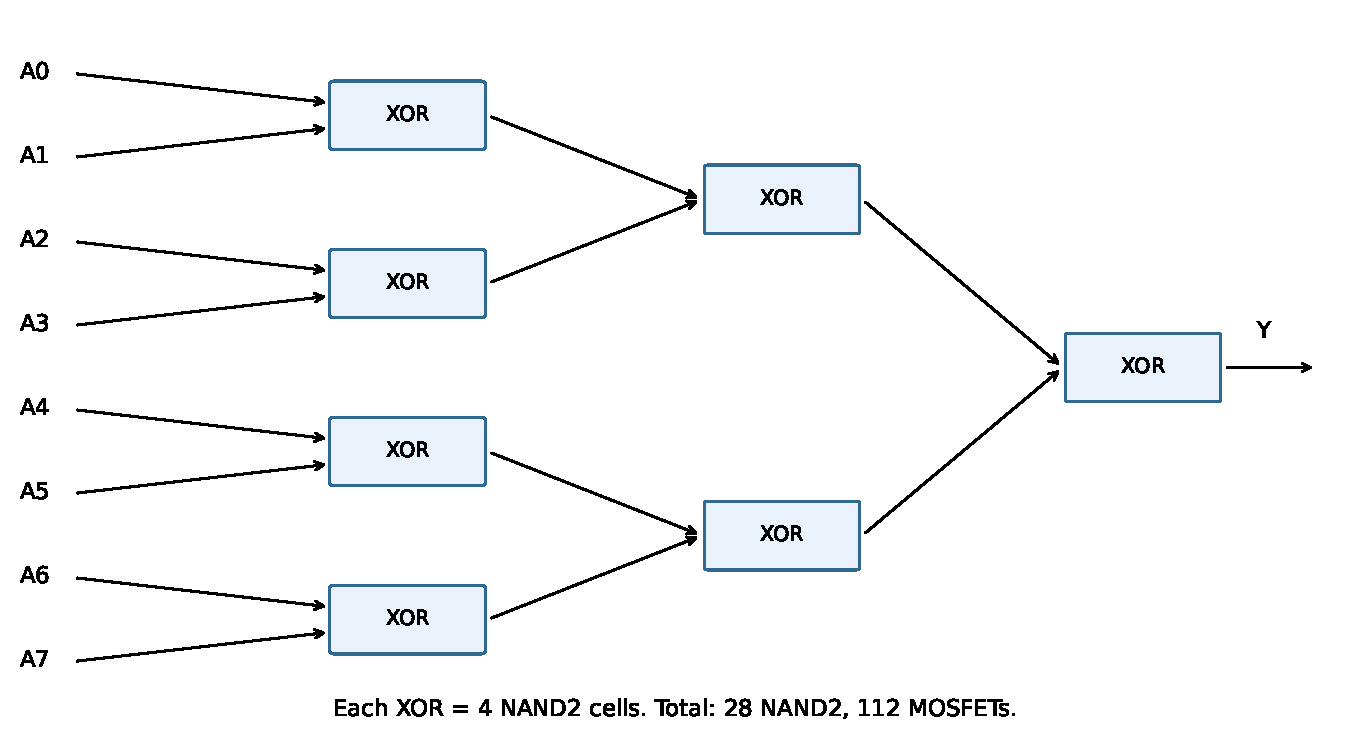
\includegraphics[width=0.85\linewidth]{figures/circuit_architecture.pdf}
\caption{Parity checker architecture (28 NAND2 gates).}
\label{fig:arch}
\end{figure}

\textbf{Definitions.}
\begin{itemize}
\item \emph{Leakage.} Leakage is the total power delivered by all independent voltage sources divided by $V_{DD}$. With inputs at exactly 0 or $V_{DD}$ this equals $-I(V_{DD})-\sum I(V_{in,high})$ in SPICE, because input sources at 0~V deliver no power. A high input also supplies gate-tunnelling current, so counting only the $V_{DD}$ supply would miss part of the leakage. In the ML prediction each transistor contributes $P=(V_d-V_s)I_d+(V_g-V_s)I_g+(V_b-V_s)I_b$ with $I_s=-(I_d+I_g+I_b)$, and the gate leakage is $\sum P/V_{DD}$. Terminal currents are signed into the terminal and measured with four separate sources: for a source written \texttt{Vd d 0 VD}, $I_d=-I(V_d)$, and likewise for the gate, source and body. KCL requires $I_d+I_g+I_s+I_b=0$ for each transistor. Closing the source current avoids a common-mode power artefact from independently predicted currents, but it does not enforce KCL at shared circuit nodes and does not guarantee positive predicted power. Summing absolute terminal currents would double-count paths and is not used. Using supply current only gives a similar mean absolute error (\SI{0.351}{\percent} against \SI{0.365}{\percent} on the gate rows), so the accuracy does not depend on this choice.
\item \emph{Corner.} A corner is one random draw of 12 values: $V_{DD}$, temperature, and five process parameters (vth0, toxe, ndep, u0, xj) for NMOS plus the same five for PMOS. All NMOS in a gate or circuit share one draw and all PMOS share another. The same 200 corners are used for the gates and for the circuit. Width is not part of the corner: it is fixed by the gate design above, as in a real sized cell. The assignment lists only $V_{DD}$, temperature and process in a corner. Width is a random variable only in the transistor datasets, which have to cover the allowed width range.
\item \emph{Relative error.} $(\mathrm{ML}-\mathrm{SPICE})/\mathrm{SPICE}$ for each gate or circuit case. We report the \emph{median} and the \emph{95th percentile} of its absolute value, the \emph{bias} (the mean signed difference ML $-$ SPICE, in nA for the tables, and the mean signed relative error where stated), and the \emph{mean accuracy} $=100\,(1-\mathrm{MAPE})$, with MAPE the mean absolute relative error. Mean accuracy is not an $R^2$ value.
\end{itemize}
